% Options for packages loaded elsewhere
\PassOptionsToPackage{unicode}{hyperref}
\PassOptionsToPackage{hyphens}{url}
%
\documentclass[
  a4paper,
  11pt,
  twocolumn]{article}
\usepackage{amsmath,amssymb}
\usepackage{iftex}
\ifPDFTeX
  \usepackage[T1]{fontenc}
  \usepackage[utf8]{inputenc}
  \usepackage{textcomp} % provide euro and other symbols
\else % if luatex or xetex
  \usepackage{unicode-math} % this also loads fontspec
  \defaultfontfeatures{Scale=MatchLowercase}
  \defaultfontfeatures[\rmfamily]{Ligatures=TeX,Scale=1}
\fi
\usepackage{lmodern}
\ifPDFTeX\else
  % xetex/luatex font selection
\fi
% Use upquote if available, for straight quotes in verbatim environments
\IfFileExists{upquote.sty}{\usepackage{upquote}}{}
\IfFileExists{microtype.sty}{% use microtype if available
  \usepackage[]{microtype}
  \UseMicrotypeSet[protrusion]{basicmath} % disable protrusion for tt fonts
}{}
\makeatletter
\@ifundefined{KOMAClassName}{% if non-KOMA class
  \IfFileExists{parskip.sty}{%
    \usepackage{parskip}
  }{% else
    \setlength{\parindent}{0pt}
    \setlength{\parskip}{6pt plus 2pt minus 1pt}}
}{% if KOMA class
  \KOMAoptions{parskip=half}}
\makeatother
\usepackage{xcolor}
\usepackage{graphicx}
\makeatletter
\def\maxwidth{\ifdim\Gin@nat@width>\linewidth\linewidth\else\Gin@nat@width\fi}
\def\maxheight{\ifdim\Gin@nat@height>\textheight\textheight\else\Gin@nat@height\fi}
\makeatother
% Scale images if necessary, so that they will not overflow the page
% margins by default, and it is still possible to overwrite the defaults
% using explicit options in \includegraphics[width, height, ...]{}
\setkeys{Gin}{width=\maxwidth,height=\maxheight,keepaspectratio}
% Set default figure placement to htbp
\makeatletter
\def\fps@figure{htbp}
\makeatother
\setlength{\emergencystretch}{3em} % prevent overfull lines
\providecommand{\tightlist}{%
  \setlength{\itemsep}{0pt}\setlength{\parskip}{0pt}}
\setcounter{secnumdepth}{5}
%------------------------------------------------------------------------------%
% PAPER TEMPLATE FOR ICPHS 2023 Prague                                         %
%                                                                              %
% Original template downloaded from:                                           %
% http://www.icphs2023.org/call-for-papers/                                    %
%                                                                              %
% Reformatted to work with Rmarkdown and R by:                                 %
% Joseph V. Casillas | Rutgers Univesity |11/11/2022                           %
%                                                                              %
% Available for download at:                                                   %
% https://github.com/jvcasillas/icphs2023_rmd_template                         %
%------------------------------------------------------------------------------%



% Packages
\usepackage{./includes/tex/icphs2023}
\usepackage{metalogo} 
\usepackage{epstopdf}
\usepackage{tipa}

% Links and urls must be black
%\hypersetup{urlcolor=black, citecolor=black, linkcolor=black}


% Packages removed from icphs2023.sty because of conflicts
% They have been added to the .Rmd yaml front matter
% \usepackage[latin1]{inputenc}
% \usepackage[T1]{fontenc}
% \usepackage[leqno,fleqn]{amsmath}
\usepackage[utf8]{inputenc}
\usepackage[T1]{fontenc}
\ifLuaTeX
  \usepackage{selnolig}  % disable illegal ligatures
\fi
\usepackage{bookmark}
\IfFileExists{xurl.sty}{\usepackage{xurl}}{} % add URL line breaks if available
\urlstyle{same}
\hypersetup{
  hidelinks,
  pdfcreator={LaTeX via pandoc}}

\author{}
\date{\vspace{-2.5em}}

\begin{document}

\title{Does immersion modality affect acquisition of the Spanish trill?}
\author{Alexander Rogers}
\organization{Rutgers University}
\email{akr122@scarletmail.rutgers.edu}


\maketitle

\begin{abstract}
This paper analyzes the production of the Spanish trill by immersion students. It analyzes the impact of different immersion modalities on the acquisition of the production of the Spanish trill.
\end{abstract}

\keywords{trill, L2A, immersion, immersion modality, acoustics, acquisition}


\section{Introduction}

The acquisition of Spanish as a second language has been studied with an
incredible diversity of approaches, points of focus, and demographics of
participants. Phoneticians have analyzed the way in which L2 learners
and bilinguals acquire such linguistic aspects as Spanish phonetic
categories, pronunciation, stress, pitch, and perception. This paper
aims to investigate a growing subfield in the world of bilingualism:
immersion. More specifically, at-home immersion school programs, and how
different modes of immersion shape the way in which L2 Spanish learners
acquire the language. Immersion schools give students the chance to live
and learn in the target language for up to their entire school day, in
some programs reaching upwards of seven hours a day. The expectation for
students of these programs is that they emerge from them able to
communicate and interact in the target language. With the variety of
immersion types and the limited number of immersion programs, however, I
think that an important question to ask is what kind of immersion works,
and to what degree. To that end, this paper is investigating how
different modalities of immersion affect the acquisition of Spanish
pronunciation, with a focus on a specific production.

\section{Background}

An important factor influencing language acquisition in an immersion
program is the modality or type of immersion. The most common types of
immersion are full (entire curriculum in the L2) and partial (up to half
of the curriculum in the L2) \cite{genesee_second_1985}. Additionally,
there are forms of immersion in which learners start fully immersed, and
have their L1 language arts introduced around 2nd or 3rd grade depending
on the district, and gradually use more and more of the L1 until around
5th grade where it becomes a partial immersion setup, with 50\% of the
curriculum in the L1 and 50\% in the L2 \cite{genesee_second_1985}.
These programs are designed with the intent to emulate L1 acquisition to
the end that the students can engage in meaningful communication in the
L2 \cite{macnamara_nurseries_1973}, though naturally different
acquisition environments mean differing results as far as student
performance and proficiency when graduating from the programs
\cite{parks_effects_2020}. While previous studies
\cite{lambert_cognitive_1969}etc. have found that students in full
immersion programs tend to perform as well as and often better than
their monolingual peers learning in fully English curriculum
\cite{campbell_review_1984} in subjects such as math, science, and
language arts, what remains to be proven is which modality of immersion
is better at teaching L2 learners to communicate in and produce the L2.

\subsection{Communication}

Communication in and production of the L2 can come in many forms. What
is of particular importance and interest to this study is Spanish
pronunciation by L2 learners. One of the greatest challenges in
acquiring additional languages is the development of speech patterns
that resemble those of native speakers of the target language
\cite{simonet_l2_2012}. Past research has found that there are many
possible factors influencing the acquisition of Spanish pronunciation.
Lenneberg \cite{lenneberg_biological_1967} popularized the critical
period hypothesis (CPH), which posits that ``the complete mastery of a
language is no longer possible if the onset of learning occurs after the
end of some period in life during which human beings retain a full
language-learning capacity'' \cite{simonet_l2_2012}. This inability to
completely acquire languages after the critical period is typically
attributed to loss of neural plasticity as the brain matures. Another
theory that attempts to explain the acquisition process of additional
languages is Flege's Speech Learning Model (SLM)
\cite{flege_second_1995}, which explains the development of phonetic
categories in language learners. Per the SLM, learners' phonetic
categories for their L1 and their L2 reside in the same cognitive space,
which allows for interaction between them when acquiring and producing
either language. This interaction can result in distinct categories for
stark phonetic productions, as well as overlap and mixing in cases when
phonetic structures are similar between languages
\cite{flege_second_1995}. While these theories and more aim to explain
how acquisition of pronunciation can occur within the individual, few
studies investigate how the context of acquisition can impact phonetic
production.

\subsection{Context of learning}

Previous studies investigating context-of-learning
\cite{simoes_phonetics_1996}, \cite{lord_combined_2000},
\cite{diaz-campos_immersion_2004} have focused on study abroad (SA) vs
at-home (AH) learning. They investigated L2 learners of Spanish in 4 to
8-week SA sessions in countries like Mexico and Spain and assessed the
degree to which context-of-learning affected nativelike pronunciation of
consonantal segments in Spanish \cite{diaz-campos_immersion_2004}. They
found that production of word-initial stops and word-final laterals
improved over the duration of the SA, and that voiced fricatives showed
little to no improvement, which they attributed to the generative
approach's idea that fricatives are more marked, and therefore more
difficult to acquire \cite{diaz-campos_immersion_2004}). This past
research leaves a gap in our understanding of the effectiveness of
context-of-learning, leaving out conventional AH vs AH immersion, and
most prominently within-immersion contexts such as full vs partial
immersion. This pilot study aims to begin to fill that gap by getting
preliminary data supporting the idea that there is a difference in
performance between full and partial immersion when it comes to L2
learner acquisition of Spanish pronunciation. Moving forward, a
full-scale study investigating this will be necessary

\subsection{Acoustics and the Spanish trill}

Many of the studies mentioned above assess Spanish pronunciation using
voice onset time (VOT) as the measure, as it is easy and simple to
measure and see differences between languages
\cite{abramson_voice-timing_1964}. For a full overview of VOT and it's
applications and usefulness in evaluating L2 Spanish pronunciation, see
studies including Flege \cite{flege_factors_1988}, Amengual
\cite{amengual_interlingual_2012}, and particularly Abramson and Whalen
\cite{abramson_voice_2017}. Though VOT is useful for investigating
native-like pronunciation of voiceless and voiced stops, this study is
looking at the pronunciation of intervocalic rhotic when producing a
trill, and thus a different measure is required. In order to analyze the
pronunciation of the trill phoneme, two measures will be used: duration
of the target sound, and number of occlusions during the trill
\cite{amengual_acoustic_2016}.

Much research has been conducted on the acquisition of the pronunciation
of Spanish vowels and consonants with many studies looking specifically
at the intervocalic rhotic trill (for a full list of studies
investigating intervocalic rhotic, see \cite{simonet_l2_2012}, which is
the phonetic feature of interest in this study. In one previous study,
Face \cite{face_intervocalic_2006} found that while L1 English learners
of Spanish were ``generally able to acquire native-like pronunciation of
Spanish tap at a relatively early age in their development
\cite{face_intervocalic_2006}, they had significantly greater
difficulties acquiring pronunciation of the Spanish trill. While they
found evidence that as proficiency and language use increased so too did
native-like pronunciation of the trill, they found that more advanced
learners tended to still overgeneralize the tap in their production of
Spanish rhotic categories. This study narrows the production tasks to
the rhotic trill in an attempt to have any variation in production rise
from the context in which the participants acquired Spanish, rather than
differentiating between rhotic categories. In another previous study,
Amengual \cite{amengual_acoustic_2016} conducted an investigation on the
acoustic correlates of the Spanish tap-trill contrast using heritage
Spanish speakers and L2 learners as participants, as a factor of
language dominance. In this study, Amengual found that Spanish-dominant
heritage speakers (SDHS) produced more canonical trills with three or
four occlusions, whereas both L2 learners and English-dominant heritage
speakers (EDHS) produced trills with one or zero occlusions. This study
proved not only that there is a significant effect of language dominance
on production of taps and trills in Spanish, but also that within one
group (heritage speakers) there can be a significant difference in
production \cite{amengual_acoustic_2016}. So the present study aims to
investigate if there is a difference between immersion learners, and
rather than dividing them by language dominance, I divided them by
immersion modality.

\section{Research questions and hypotheses}

For this project, I sought to answer three research questions. First,
among a small group of L1 English speakers who participated in immersion
programs, can different immersion modalities (partial, full) influence
the way in which they acquire the Spanish trill? And lastly, to what
degree are the participants able to approximate the native pronunciation
of the Spanish trill? Following previous research which has proven that
immersion abroad is more effective than typical AH learning, I
hypothesize that full immersion will be more effective than partial
immersion in training L2 learners of Spanish to have native-like
pronunciation of /r/. I also hypothesize that different immersion
modalities will have a significant impact on acquisition of
pronunciation and production in Spanish. I expect more time immersed in
the language to result in better production values and more native-like
trill duration and occlusions. With those hypotheses in mind, I expect
that there will still be a noticeable difference between L2 learners and
native speakers. As has been found previously \cite{flege_factors_1988}
etc., age of acquisition is one of the most important factors when
creating phonological categories, regardless of context of learning, and
all of the participants started learning Spanish around five or six
years of age.

\section{Procedure}

\subsection{Participants}

Because this is a rather small pilot version of the study, there are
only 5 participants. I had intended for there to be at least one more so
I could have 2 of each participant group (full immersion, partial
immersion, native speaker) but there were some issues getting data from
a few participants. In the end, I have 2 participants who attended full
immersion (FI) programs, 1 who attended a partial immersion (PI)
program, and 2 native speakers. All of the participants from immersion
programs are from the United States. The full immersion participants are
both 25 years old, 1 male and 1 female. The partial immersion
participant is a 27 year old male. The native speakers are 26 and 28
years old, both male, one from Spain and one from Chile.

\subsection{Methods}

This project consists of two tasks: a language use and socioeconomic
status questionnaire, namely, the LEAP-Q \cite{marian_leapq_2007}
followed by a speech production task in the form of sentence reading.
The LEAP-Q questionnaire was chosen for a number of reasons. Chief among
them is its widespread use and recognition within the field of
sociolinguistics, as well as linguistics as a whole. This allowed me to
use it without having to make changes or to attempt to design my own
questionnaire, which would have been too difficult for this project.
Furthermore, the LEAP-Q is a very comprehensive questionnaire covering
social background, language use and dominance, education level, and
more, which are all very useful points of information for me.

The second task, the sentence reading and production task, was chosen
because it is a straightforward and simple way to elicit the desired
phonetic structures remotely, as the participants are in cities across
the US while I am in New Jersey. They were sent a set of five stimulus
sentences, each having the target word embedded within a sentence in
order to elicit the most naturalistic pronunciation possible from the
participants. Each target word contained the double /r/ trill, and there
were no other trills within the stimuli. The participants recorded
themselves saying the sentences out loud, one after the other, within
one sound file.

The data were all segmented in Praat \cite{boersma_praat_2001} before
having the target phoneme's duration and number of occlusions measured.
The analysis in Praat was conducted following Amengual
\cite{amengual_acoustic_2016}'s approach, by measuring the number of
occlusions and the overall duration of the rhotic segment (in
milliseconds, ms). An occlusion was determined to have occurred when
lingual contact, a reduction in the amplitude of the waveform, a
transition in F3 and F4 formant structure, and changes in intensity were
observed. The actual analysis was done in R-studio. Duration and
occlusion count averages were grouped by L1 (English or Spanish) and by
immersion mode (full or partial) and plotted. Future work on this topic
will conduct statistical analysis and model the effects being
investigated.

\section{Results}

Based on the analysis mentioned above, I was able to get a (very
generalized) idea of how /r/ duration and number of occlusions differs
both between immersion modalities and between native language speakers.
Table 1 contains the descriptive statistical information for each
participant. For all of the stimuli together, the full immersion
participants had a mean number of occlusions of 1.2, the partial
immersion participants had 0.4, and the native speakers had 2.125. The
FI participants had a mean /r/ duration of 0.0551 seconds, the PI
participants had 0.0416 seconds, and the native speakers had 0.0807
seconds. Figure 1 shows the distribution of duration and occlusion
measurements for each participant, and Figure 2 shows the averages.

\begin{figure}[!ht]
\begin{center}
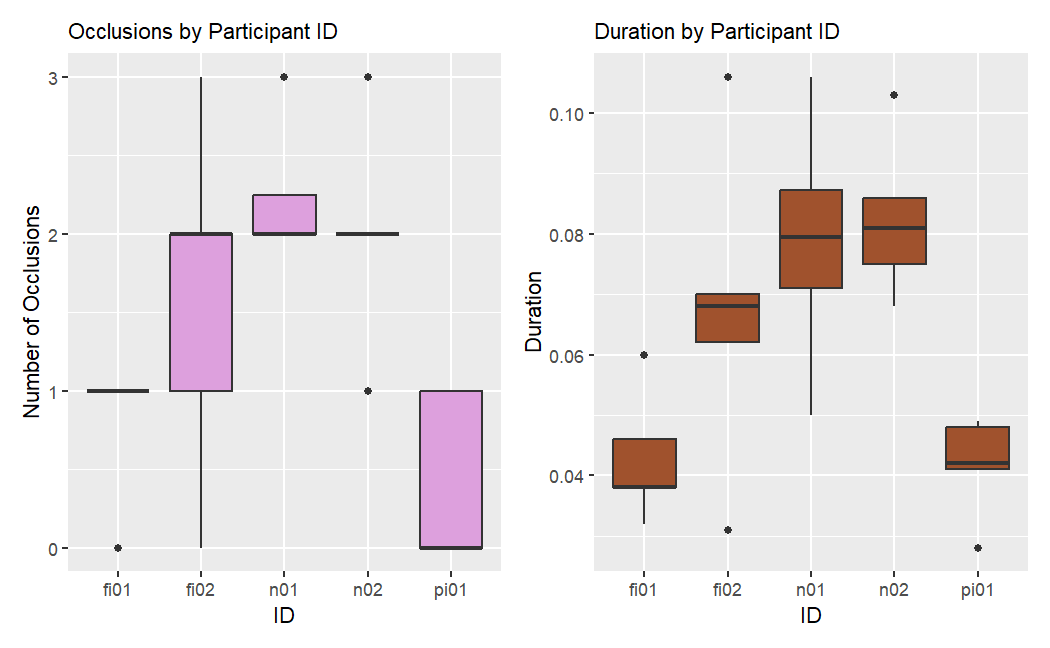
\includegraphics[width=6cm]{./includes/figures/fig1.png}
\caption{Distributions by duration and number of occlusions.}\label{fig:Distributions}
\end{center}
\end{figure}

\section{Discussion and conclusions}

I'm going to begin the discussion with a disclaimer: because the sample
size for this project is so small, the results cannot and should not be
taken as a generalization for all immersion learners, and will not be
truly representative of the wider population of which a small sample
were studied here. That being said, I think that the data found here
make for a very interesting starting point for further investigation.\\
In this study, I sought to investigate whether immersion modality had an
impact on the acquisition of the Spanish trill. And since the quality of
the trill cannot really be evaluated here without comparing it to the
productions of the native speaker participants, I will tie in my other
research question here as well. That being evaluating the degree to
which the L2 learner participants were able to produce a native-like
trill. Looking back to figures 1 and 2, we can see that the full
immersion (FI) participants had overall more occlusions and longer
durations than the partial immersion (PI) participants. Furthermore,
though neither FI participant ever quite reached the level of
native-like production, they were consistently closer than the PI
participant. From this, we can see that (for the very small sample size
used here) L2 Spanish learners who attended a full immersion program had
an advantage in trill production. I think that even with this very
limited study, the results are interesting and show that this is a
question worth further investigation. In the future, I would like to
re-conduct this study with a participant pool of sufficient power to
derive actual, informative results from the study. Additionally, for
that study I would like to be better prepared for statistical analysis,
at least to the point where I would be able to conduct an ANOVA or
random effect model. I truly believe that, properly conducted, this will
be a very interesting study with a lot of potential to improve the
immersion education model.

\begin{figure}[!ht]
\begin{center}
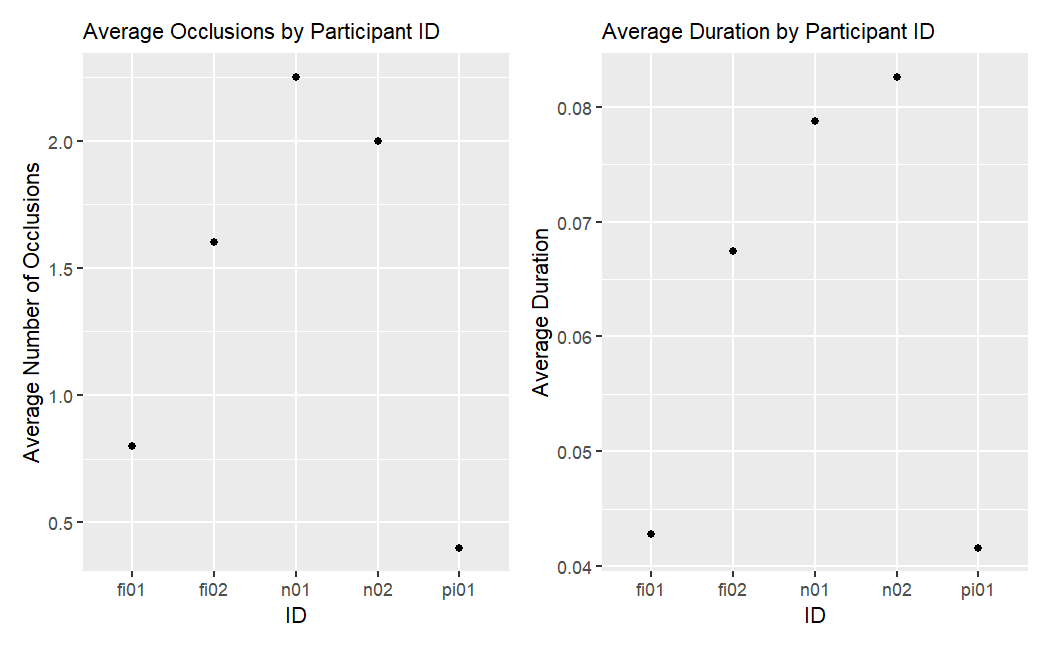
\includegraphics[width=6cm]{./includes/figures/fig2.png}
\caption{Mean durations and number of occlusions.}\label{fig:Means}
\end{center}
\end{figure}

\bibliographystyle{./includes/bib/IEEEtran.bst}
\bibliography{./includes/bib/phonobib.bib}

\theendnotes

\end{document}
